\section{System design}
\label{sec:system}

\paragraph{Architecture overview.}
Figure~\ref{fig:architecture} separates the client interface, local orchestration and editing core, remote model boundary, and persistent media and revision state. The browser submits briefs and follow-up requests through FastAPI; the editing workflow builds a source-linked plan, while the local media pipeline validates and renders it. Model calls are budgeted separately from deterministic media operations. Optional interfaces and the RSI extension are distinguished from the B2 path used in the recorded comparison.

\begin{figure}[htbp]
\centering
% Keep supplied raster artwork intact. Crop the embedded heading and use
% LaTeX overlays to correct terminology without repainting the source asset.
\begingroup%
\setlength{\unitlength}{\dimexpr\linewidth/1376\relax}%
\begin{picture}(1376,690)%
\put(0,0){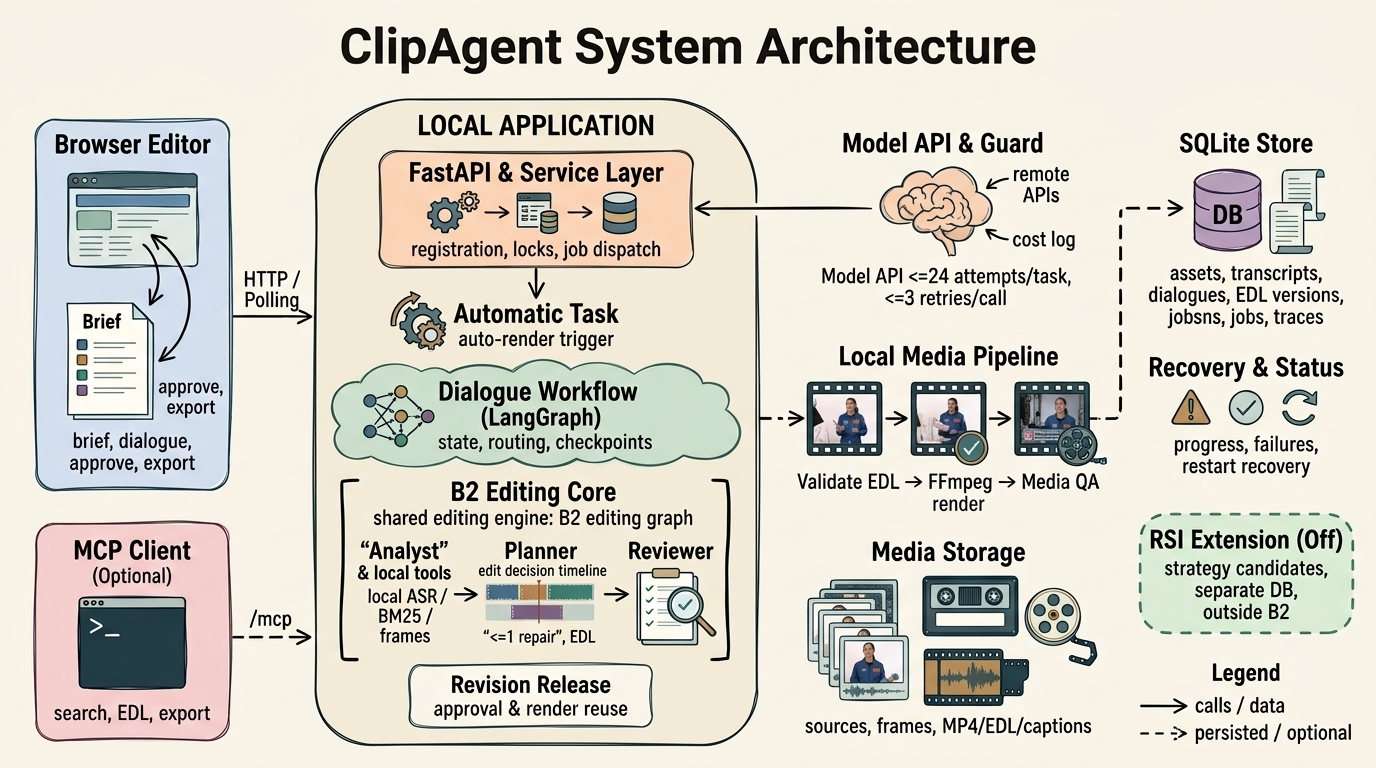
\includegraphics[width=\linewidth,trim=0 0 0 78,clip]{figures/architecture-original.jpeg}}%
\put(807,449){\color{diagramcream}\rule{310\unitlength}{64\unitlength}}%
\put(807,449){\makebox(310,64){\sffamily\fontsize{6.2}{7.4}\selectfont\shortstack{Model API: $\leq 24$ attempts/task\\$\leq 3$ attempts/call (incl. retries)}}}%
\put(1157,430){\color{diagramcream}\rule{199\unitlength}{75\unitlength}}%
\put(1157,430){\makebox(199,75){\sffamily\fontsize{6.0}{7.2}\selectfont\shortstack{Assets, transcripts,\\dialogue, EDL versions,\\jobs and traces}}}%
\end{picture}%
\endgroup%
\caption{ClipAgent system architecture. The local application coordinates dialogue and the shared B2 editing core; remote model calls cross an explicit API boundary, while rendering and media checks run locally. SQLite retains revision and task state. The optional MCP interface and disabled-by-default RSI extension are outside the evaluated B2 configuration. The guard permits at most 24 model HTTP attempts per foreground task and three attempts per call, including retries.}
\label{fig:architecture}
\end{figure}
\paragraph{Preparation and evidence retrieval.}
FastAPI starts and polls asynchronous tasks. Local faster-whisper base \citep{fasterwhisper} transcribes speech with timestamps. BM25 retrieves related transcript spans. An analysis role in LangGraph can read source intervals and inspect sampled frames when the brief requires visual evidence. Local audio processing reduces data sent to remote services. The configured planning and vision endpoints can receive the brief, transcript evidence and sampled frames.

\paragraph{Planning, review, and execution.}
The planning role combines the brief, prior edit, conversation state and tool observations to choose source intervals, order, duration, aspect ratio and subtitle settings. A separate reviewer checks the EDL and can request one repair with a concrete issue. Pydantic schemas and deterministic validators check source bounds, overlap and format constraints. FFmpeg \citep{ffmpeg} executes a validated EDL and checks decoded media, duration, dimensions and subtitle availability. The task record preserves source timecodes and evidence identifiers. Prompts and tool schemas are in \path{app/services/editing_agent.py}, orchestration in \path{app/graph/editing.py}, and rendering in \path{app/services/renderer.py}.


Figure~\ref{fig:workflow} details the editing loop within this architecture. Evidence acquisition supplies timed speech and, when needed, sampled frames. The planner proposes an EDL and the independent reviewer can request at most one semantic repair. A reviewed plan must still pass deterministic validation before FFmpeg renders it; media QA then checks the output. Persisted revision context supports subsequent edits, and approval remains bound to the selected revision rather than to the conversation as a whole.

\begin{figure}[htbp]
\centering
% Remove the artwork's baked-in "Figure 1" heading; numbering belongs to LaTeX.
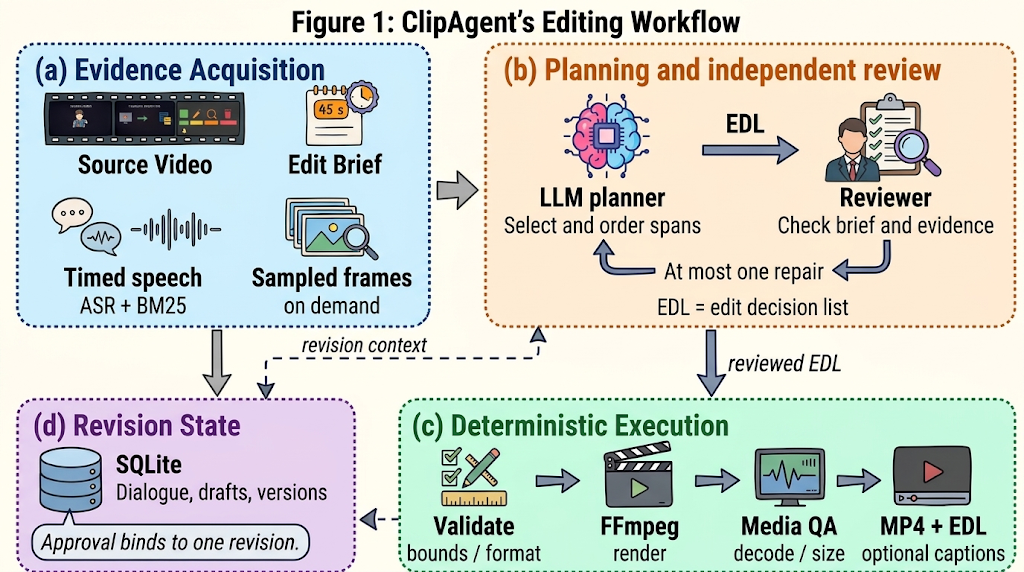
\includegraphics[width=0.88\linewidth,trim=0 0 0 39,clip]{figures/workflow-original.png}
\caption{Evidence-grounded editing workflow. (a) Timed transcript retrieval and on-demand frames ground the brief. (b) The planner selects and orders source spans; an independent reviewer checks the proposal and may request one repair. (c) Deterministic validation, FFmpeg rendering and media QA produce the MP4 and source-linked EDL, with optional captions. (d) SQLite stores dialogue, drafts and versions, providing revision context for follow-up requests.}
\label{fig:workflow}
\end{figure}
\FloatBarrier

\paragraph{State and recovery.}
An explicit requirement overrides prior revision settings and confirmed aspect-ratio or subtitle defaults. SQLite stores drafts, dialogue, tasks and versions. Approval binds to a revision and can reuse a completed render. The isolated restart test restored drafts and downloads, rejected stale approval with HTTP 409, and marked an injected queued task interrupted with a structured error. A missing asset returned HTTP 404. Each foreground task limits model HTTP attempts to 24 across all roles and vision, with at most three attempts per call. Retries count toward this budget because repeated requests can incur additional charges. The UI reports exhausted budgets and failed tasks.

\paragraph{Optional strategy adaptation.}
The RSI module records eligible feedback in a separate database and proposes structured strategy candidates with bounded background work. Offline evaluation and manual activation control which strategies may enter eligible planning prompts. Model weights, tool permissions and validators remain fixed. RSI defaults off and is disabled by the comparison runner. The recorded study predates this module. Automated tests exercise activation, isolation, fallback, and budget exhaustion.

\FloatBarrier
